
\section{Model}

\begin{frame}
    \frametitle{Stochastics}
	\begin{itemize}
		\item Brownian Motion (Random Walks) - $W(t)$
		\item Properties
	\begin{enumerate}[i]
		\item $W(t)$ is continuous
		\item $W(t)$ is no where differentiable
		\item If $t_{1}<t_{2}<t_{3}<t_{4}$, \\
			$W(t_{1}), W(t_{2})-W(t_{1}),  W(t_{3})-W(t_{4})$ are independent random variables
		\item If $0 \le s\le t$ then $W(t)-W(s) \sim N(0, t-s)$
	\end{enumerate}
		\item Gaussian White ``Noise" - $dW$
	\end{itemize}
%%%%%%%%%% Brownian Motion, Gaussian White Noise
\end{frame}



\begin{frame}
    \frametitle{Models}
	\begin{eqnarray}
		dx &=& \tilde{r} x \left( 1- \frac{x}{\tilde{f}}\right) dt +\alpha x \, dW \\
		dm &=& ( \rho m - \beta x + P) dt - \gamma x \, dW
	\end{eqnarray}
	\begin{itemize}
		\item Known Parameters - $\tilde{r}$, $\tilde{f}$, $\rho$, $\beta$
		\item Unknown Parameters - $\alpha$, $\gamma$, $P$
	\end{itemize}
\end{frame}




\section{Numerics}

\begin{frame}
   \frametitle{Approximation}
%%%%%%%%%Include figure
\vspace*{-3em}
	\begin{eqnarray*}
		dX &=& f(X) \, dt + g(X) \, dW \\
	\end{eqnarray*}
\vspace*{-3em}
	\begin{center}
		$X_{j} =$ approximation of $X(t_{j})$ \\ [20pt]
	\includegraphics[height=4cm]{approximation}
	\end{center}

\end{frame}



\begin{frame}
    \frametitle{Methods of Approximations}
	Euler-Maruyama Method - $O(\Delta t^{1})$
	\begin{eqnarray*}
		X_{j} &=& X_{j-1} + f(X_{j-1})\triangle t+ g(X_{j-1})(W(\tau_{j})-W(\tau_{j-1})) \\
		 j &=& 1,2,... ,L \\
	\end{eqnarray*}
	Milstein Method - $O(\Delta t^{1.5})$
	\begin{eqnarray*}
		X_{j} &=& X_{j-1} + \triangle tf(X_{j-1}) + g(X_{j-1})(W(\tau_{j})-W(\tau_{j-1})) 	\nonumber\\ 
		&& + \frac{1}{2} g(X_{j-1})g'(X_{j-1})((W(\tau_{j})-W(\tau_{j-1}))^{2}-\triangle t)\\
		 j &=& 1,2,... ,L \\
	\end{eqnarray*}
\end{frame}


\begin{frame}
    \frametitle{Benchmark}
	\framesubtitle{Paths}
\hspace*{-2cm}
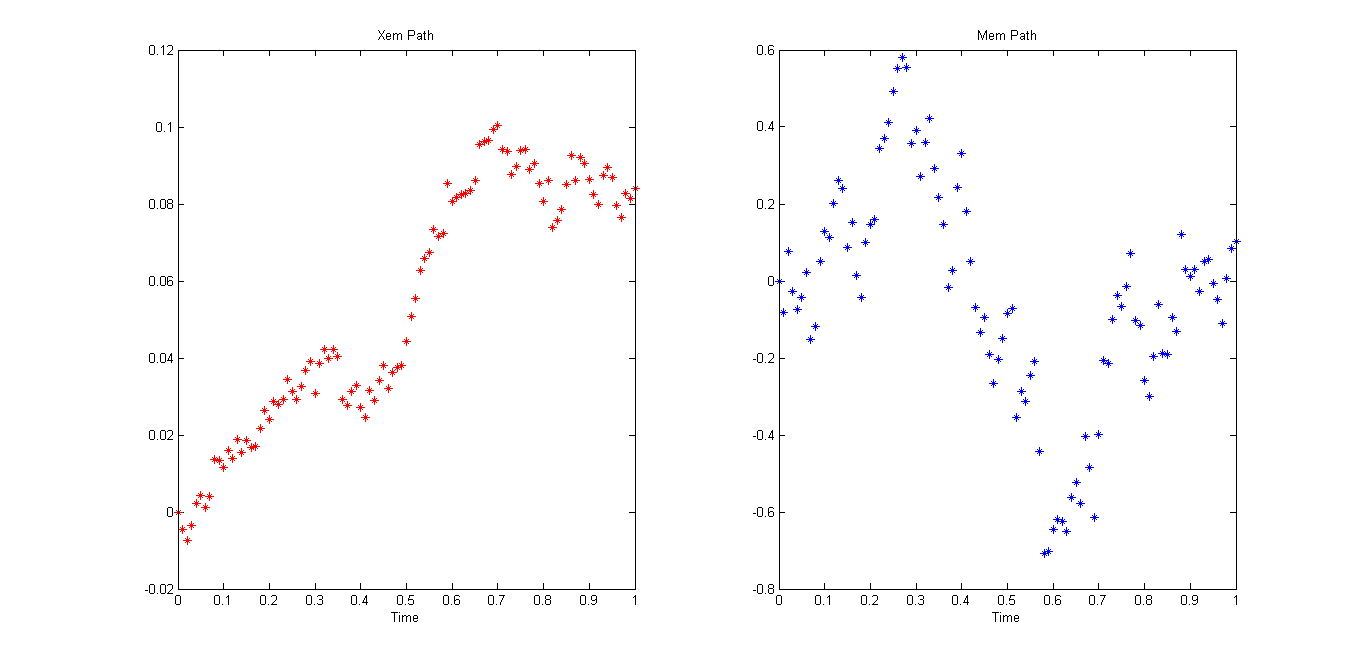
\includegraphics[height=7cm]{testpaths} 
\end{frame}


\begin{frame}
    \frametitle{Benchmark}
	\framesubtitle{Histogram}
\hspace*{-5mm}
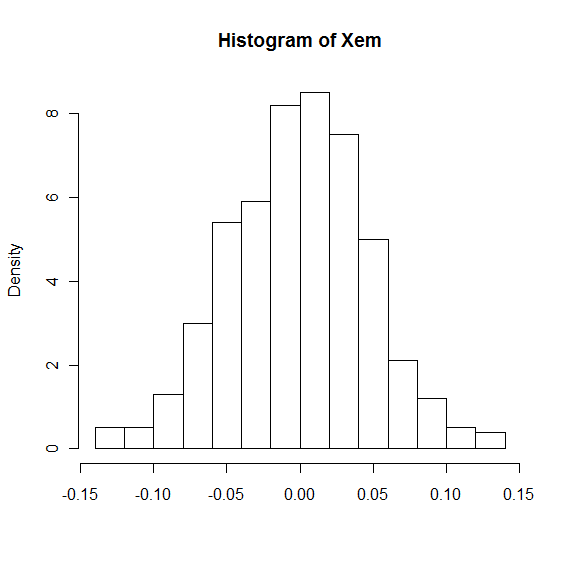
\includegraphics[height=6cm]{testhistX}
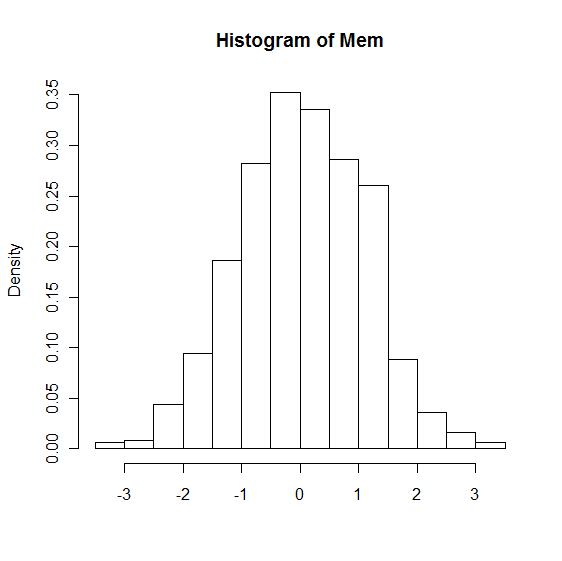
\includegraphics[height=6cm]{testhistM}
\end{frame}


\begin{frame}
    \frametitle{Benchmark}
	\framesubtitle{95\% Confidence Interval}
\begin{center}
	$\bar{x} \pm t_{(\alpha /2, df=n-1)} \frac{s}{\sqrt{n}}$ \\ 
\vspace{5mm}
\begin{tabular}{r c l c r c l}
	$E[X]$ &=& 0 && $E[M]$ &=& 0 \\
	$Var[X]$ &=& 0.0025  && $Var[M]$ &=& 1 
\end{tabular}
\end{center}
\begin{itemize}
	\item $\bar{X}$ (-0.0088, 0.0067)
	\item $\bar{M}$ (-0.137, 0.217)
\end{itemize}
\end{frame}


\begin{frame}
    \frametitle{Parameter Space}
%%%%%%%%%% Include 3D plot of parameter space
\end{frame}



